% Before, finding the critical points of \equationautorefname~\eqref{eq:AutonomousSystemODEs}, we fix the parameter, $T$, to the optimal temperature, $12.5^{\circ}$C, eliminating the effect of temperature on the salmon population.
% We can also rewrite the equations in a similar form to Theodore Modis' model, as shown below,
% \begin{equation}
%     \begin{aligned}
%     \frac{dx}{dt} &= R(T_{opt})x -\frac{R(T_{opt})x^2}{K_x} - c_{xy}xy,\\[.4cm]
%     \frac{dy}{dt} &=r_yy -\frac{r_yy^2}{K_y} + c_{yx}xy.
%     \end{aligned}
% \end{equation}
% Then, substituting $ a_x = R(T_{opt})=0.47$, $\displaystyle b_x = \frac{R(T_{opt})}{K_x}=0.0313$, $a_y = r_y=0.044$, and $\displaystyle b_y = \frac{r_y}{K_y}=.0088$ we get
% \begin{equation}\label{eq:AutonomousSystemODEsModis}
%     \begin{aligned}
%     \frac{dx}{dt} &= a_xx - b_xx^2 - c_{xy}xy,\\
%     \frac{dy}{dt} &= a_yy - b_yy^2 + c_{yx}xy.
%     \end{aligned}
% \end{equation}
We find the critical points by setting the rate functions in \equationautorefname~\eqref{eq:AutonomousSystemODEsModis} to 0,
\begin{equation*}
    \begin{aligned}
    0 &= x(a_x - b_xx - c_{xy}y),\\
    0 &= y(a_y - b_yy + c_{yx}x).
    \end{aligned}
\end{equation*}
Then, we solve for $x$ and $y$ to get the following critical points;
\begin{equation*}
    \begin{array}{llll}
         x^*_1 = 0, &&& y^*_1 = 0,  \\[.2cm]
         x^*_2 = \scalebox{1.3}{$\frac{a_x}{b_x}$}= K_x,&&& y^*_2 = 0,\\[.2cm]
         x^*_3 = 0, &&& y^*_3 = \scalebox{1.3}{$\frac{a_y}{b_y}$}=K_y,\\[.2cm]
         x^*_4 = \scalebox{1.3}{$\frac{a_xb_y-c_{xy}a_y}{c_{xy}c_{yx}+b_xb_y}$}, &&& y^*_4 = \scalebox{1.3}{$\frac{a_xc_{yx}+b_xa_y}{c_{xy}c_{yx}+b_xb_y}$}.
    \end{array}
\end{equation*}
We can determine the stability at each of the above critical points by finding the eigenvalues of our model, \equationautorefname~\eqref{eq:AutonomousSystemODEsModis}~\cite{roussel2019stability}.
We begin by constructing the Jacobian matrix,
\begin{equation}\label{eq:Jacobian}
    J_{(x,y)} =
    \begin{pmatrix}
        a_x - 2b_xx -c_{xy}y & -c_{xy}x\\
        c_{yx}y & a_y - 2b_yy + c_{yx}x
    \end{pmatrix}.
\end{equation}
Then, we derive the characteristic polynomial,
\begin{align}
\begin{split}\label{eq:CharacteristicEq}\displaystyle
    \text{det}(J_{(x,y)}-\lambda I) = \lambda^2 - \pmb{\big[}\; (a_x - 2b_xx -c_{xy}y) + (a_y - 2b_yy + c_{yx})\;\pmb{\big]}\lambda\\
    + \pmb{\big[}\; (a_x - 2b_xx -c_{xy}y)(a_y - 2b_yy + c_{yx}) + c_{xy}xc_{yx}y\;\pmb{\big]}.
\end{split}
\end{align}
Note that the trace and determinant of the Jacobian matrix are
\begin{equation*}
    \begin{array}{ll}
         \mathrm{T} &= \text{tr}(J_{(x,y)}) = (a_x - 2b_xx -c_{xy}y) + (a_y - 2b_yy + c_{yx}),
         \\
         \mathrm{D} &= \text{det}(J_{(x,y)}) = (a_x - 2b_xx -c_{xy}y)(a_y - 2b_yy + c_{yx}) + c_{xy}xc_{yx}y.
    \end{array}
\end{equation*}
So, substituting the above variables in \equationautorefname~\eqref{eq:CharacteristicEq} produces
\begin{equation*}
    \text{det}(J_{(x,y)}-\lambda I) = \lambda^2 - \mathrm{T}\lambda + \mathrm{D}.
\end{equation*}
Now, solving for our eigenvalues, $\lambda$, gives the below equation,
\begin{equation*}
    \lambda = \frac{\mathrm{T} \pm \sqrt{\mathrm{T}^2 - 4\mathrm{D}}}{2}.
\end{equation*}
Using the equation above, we can determine the signs and potentially the numeric values of the real and imaginary parts of the eigenvalues for each critical point.
Starting with the first critical point, $(0,\;0)$, we get
\begin{equation*}
    \begin{array}{l}
         \mathrm{T}= a_x+a_y, \\
         \mathrm{T}^2 - 4\mathrm{D}= (a_x-a_y)^2 .
    \end{array}
\end{equation*}
So, substituting in the values for $a_x$ and $a_y$, we get
\begin{equation*}
    \begin{array}{l}
         \mathrm{T} = \ln(0.32*5) + 0.059 \approx 0.529,  \\
         \mathrm{T}^2-4\mathrm{D} = (\ln(0.32*5)-0.059)^2 \approx 0.169.
    \end{array}
\end{equation*}
Since $\mathrm{T}\approx 0.529 > \sqrt{\mathrm{T}^2-4\mathrm{D}} \approx 0.411$, both eigenvalues are positive real values, which implies that the first critical point is an unstable node. Now, for the second critical point, $\displaystyle\left(\frac{a_x}{b_x},\;0\right)$, we get
\begin{equation*}
    \begin{array}{l}
        \mathrm{T}= a_x \left(\scalebox{1.3}{$\frac{c_{yx}}{b_x}$}-1\right)+a_y, \\[.2cm]
        \mathrm{T}^2 - 4\mathrm{D}= \scalebox{1.3}{$\frac{(a_x (b_x+c_{yx})+a_y b_x)^2}{b_x^2}$},
    \end{array}
\end{equation*}
where the stability is dependent on $c_{yx}$.
Because the value for the discriminant is squared, it is always positive, which implies that the eigenvalues are real.
When we substitute the parameters, $a_x,\;b_x,$ and $a_y$ for their numeric values, we get the following criterion;
\begin{equation*}
    \begin{array}{l}
        \mathrm{T}+\sqrt{\mathrm{T}^2-4\mathrm{D}}>0,  \\
         \mathrm{T}-\sqrt{\mathrm{T}^2-4\mathrm{D}}<0.
    \end{array}
\end{equation*}
This implies that one eigenvalue is positive while the other is negative, which makes $\displaystyle\left(\frac{a_x}{b_x},\;0\right)$ a saddle point.
% for any $c_{yx}>0$. 
Now, looking at the third critical point, $\displaystyle\left(0,\;\frac{a_y}{b_y}\right)$, the trace and discriminant are;
\begin{equation*}
    \begin{array}{l}
        \mathrm{T}= a_x-\scalebox{1.3}{$\frac{a_y (b_y+c_{xy})}{b_y}$}, \\[.2cm]
        \mathrm{T}^2 - 4\mathrm{D}= \scalebox{1.3}{$\frac{(a_x b_y+a_y (b_y-c_{xy}))^2}{b_y^2}$},
    \end{array}
\end{equation*}
where the stability is now dependent on $c_{xy}$.
Just like for the last critical point, the discriminant is always positive, which implies the eigenvalues are also real.
Then, we substitute the values for, $a_x,\;a_y,$ and $b_y$, into the above equations to get the criterion below;
\begin{equation*}
    \begin{array}{l}
        \mathrm{T}+\sqrt{\mathrm{T}^2-4\mathrm{D}}>0\ \ \text{when \ } c_{xy}<0.094,  \\
        \mathrm{T}-\sqrt{\mathrm{T}^2-4\mathrm{D}}<0.
    \end{array}
\end{equation*}
From the signs of the eigenvalues, we determine that $\displaystyle\left(0,\;\frac{a_y}{b_y}\right)$ is a saddle point when $c_{xy}<0.094$, and a stable node when $c_{xy}>0.094$.
Lastly, with the critical point,
\begin{equation*}
    \left(x_4^*,\;y_4^*\right) = \left(\scalebox{1.3}{$\frac{a_xb_y-c_{xy}a_y}{c_{xy}c_{yx}+b_xb_y}$},\; \scalebox{1.3}{$\frac{a_xc_{yx}+b_xa_y}{c_{xy}c_{yx}+b_xb_y}$}\right),
\end{equation*}
we get the following trace and discriminant equations;
\begin{equation*}
    \begin{array}{l}
        \mathrm{T}= \scalebox{1.3}{$\frac{a_y b_x (c_{xy}-b_y)-a_x b_y (b_x+c_{yx})}{b_x b_y+c_{xy} c_{yx}}$}, \\[.3cm]
        \begin{aligned}
            \mathrm{T}^2 - 4\mathrm{D}=& \scalebox{1.3}{$\frac{(a_y b_x (c_{xy}-b_y)-a_x b_y (b_x+c_{yx}))^2}{(b_x b_y+c_{xy} c_{yx})^2}$}\\[.2cm]
            &- \scalebox{1.3}{$\frac{4 (a_x c_{yx}+a_y b_x) (a_x b_y-a_y c_{xy}) (b_x b_y+c_{xy} c_{yx})}{(b_x b_y+c_{xy} c_{yx})^2}$},
        \end{aligned}
    \end{array}
\end{equation*}
where the stability is dependent on parameters, $c_{xy}$ and $c_{yx}$.
Since the other critical points contain one or more species with a population size of 0, we construct the following constraints for the critical point;
\begin{equation*}
    x_4^* = \scalebox{1.3}{$\frac{a_xb_y-c_{xy}a_y}{c_{xy}c_{yx}+b_xb_y}$}>0,\quad \text{and}\quad y_4^* = \scalebox{1.3}{$\frac{a_xc_{yx}+b_xa_y}{c_{xy}c_{yx}+b_xb_y}$}>0,
\end{equation*}
which eliminates the chance of repeating any of the first 3 critical points.
From the above constraint, we create the below criterion for $c_{xy}$ and $c_{yx}$;
\begin{equation*}
\begin{array}{c}
     0<c_{xy} < \scalebox{1.3}{$\frac{a_xb_y}{a_y}$}, \\[.1cm]
     c_{yx} > -\scalebox{1.3}{$\frac{b_xa_y}{a_x}$}.
\end{array}
\end{equation*}
Since $a_x,\;b_x,\;a_y>0$, the criterion changes to
\begin{equation*}
\begin{array}{c}
     0<c_{xy} < \scalebox{1.3}{$\frac{a_xb_y}{a_y}$} \approx 0.094, \\
     c_{yx} > 0.
\end{array}
\end{equation*}
The values for the discriminant, $\mathrm{T}^2-4\mathrm{D}$, and trace, $\mathrm{T}$, can be plotted by designing a meshgrid for the parameters $c_{xy}$ and $c_{yx}$ based on their constraints as shown below.
\begin{figure}[H]
    \centering
    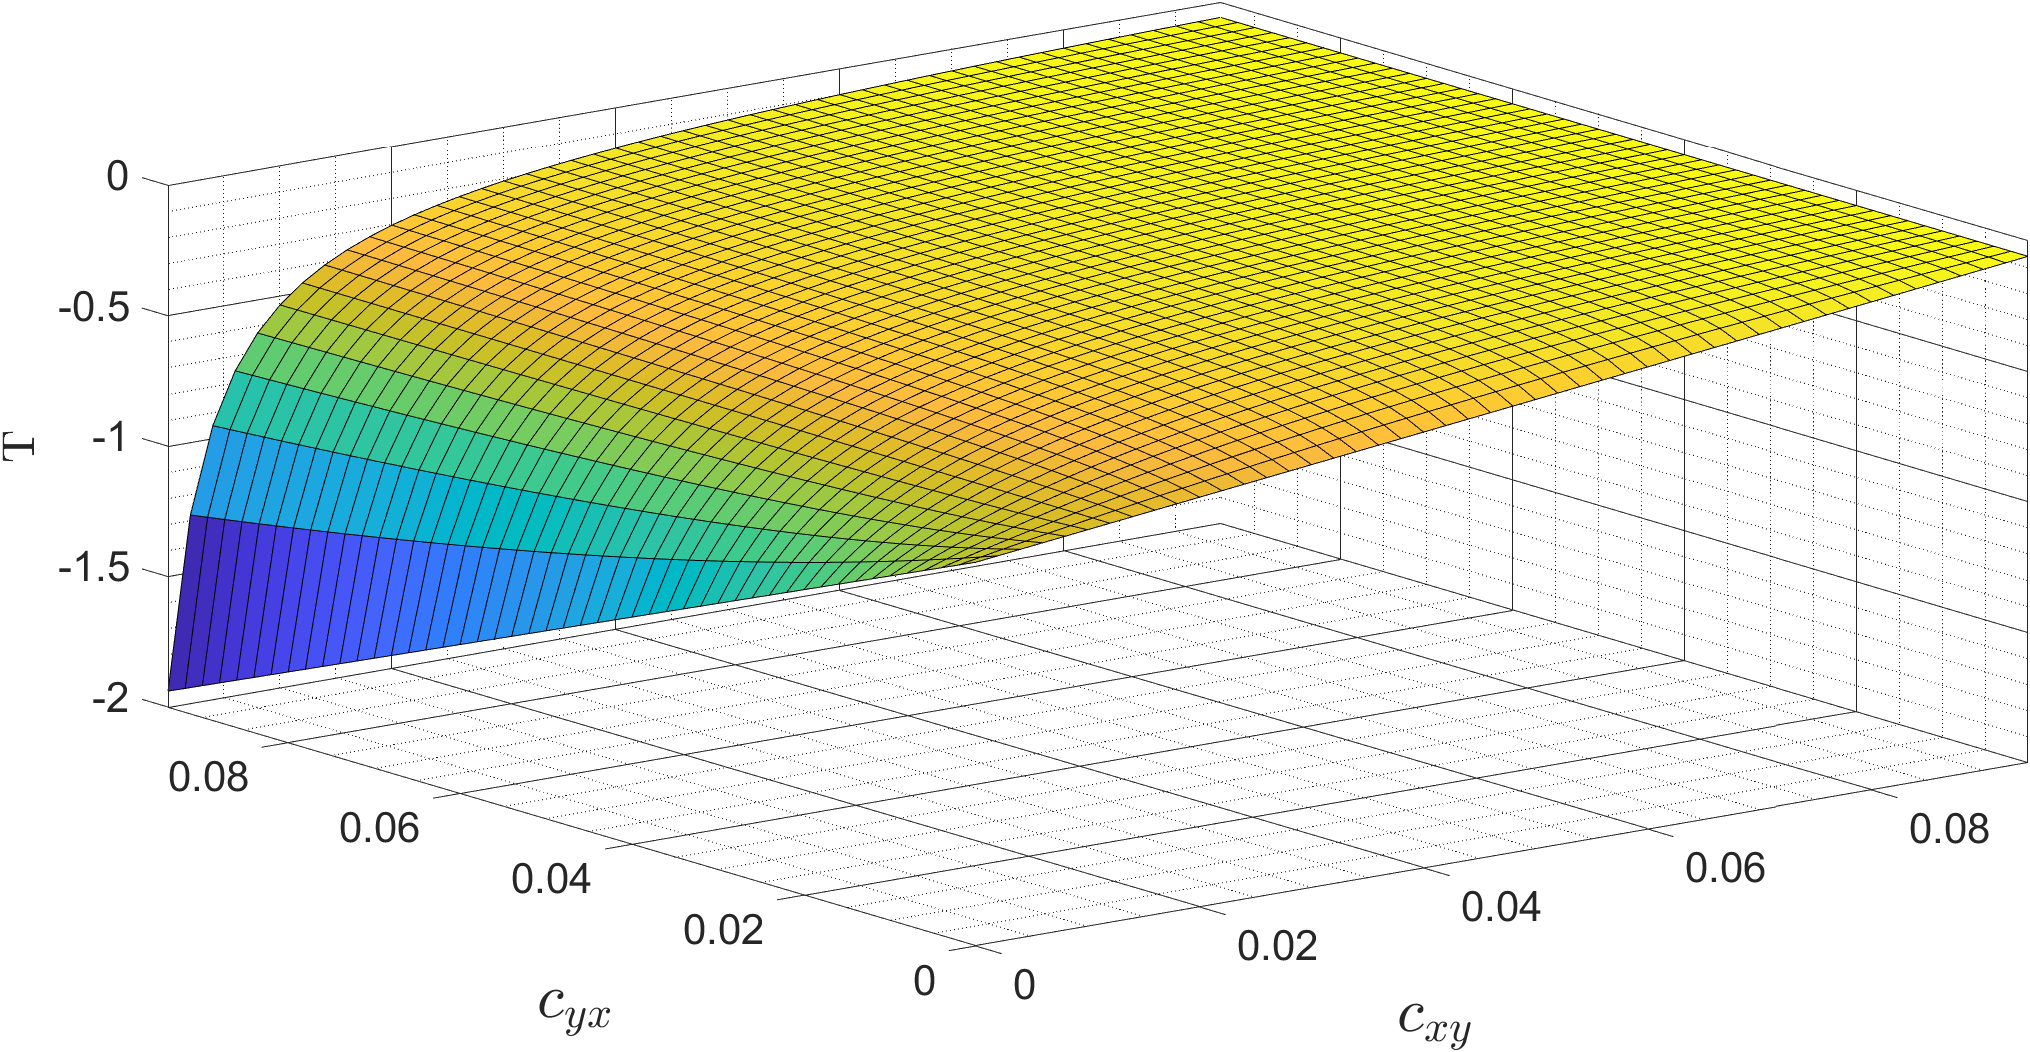
\includegraphics[width=14cm]{Pictures/Stability/Trace.png}
\end{figure}
\begin{figure}[H]
    \centering
    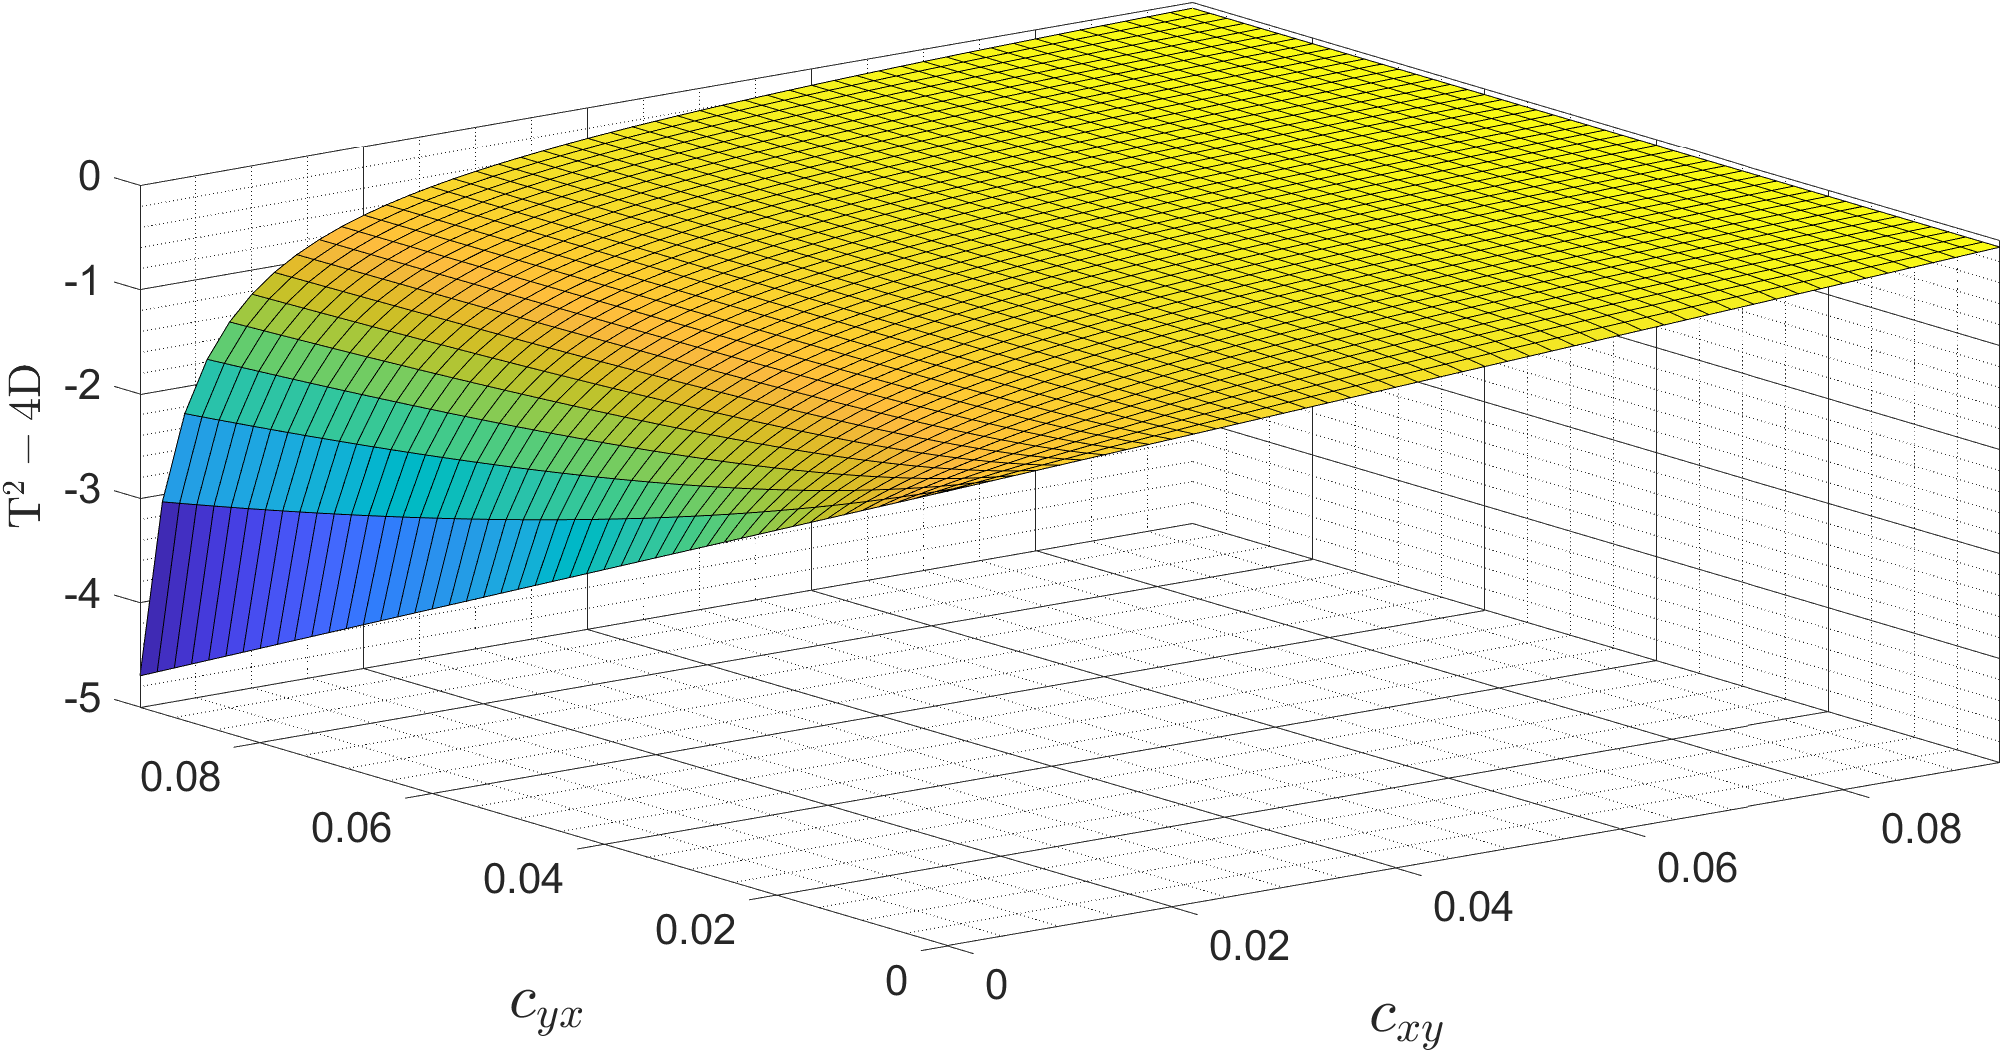
\includegraphics[width=14cm]{Pictures/Stability/Discriminant.png}
    \caption{\singlespacing
    The graphs above are the trace and discriminant of $\displaystyle J_{(x^*_4,y^*_4)}$ for different values of the parameters $c_{xy}$ and $c_{yx}$.}
    \label{fig:TraceDiscriminant}
\end{figure}
Notice that the trace and discriminant values are always negative for all $c_{xy}$ and $c_{yx}$ that belong in their constraints.
If we assume that $c_{yx}>c_{xy}$, then we are stating that the impact of salmon on brown bears is greater than brown bears on salmon.
However, brown bears eat a large quantity of salmon yearly, which means to support a brown bear's diet, there would need to be an abundance of salmon, whereas one brown bear kills thousands of salmon yearly ~\cite{deacy2018phenological,hilderbrand1999effect}.
So, the brown bear population should have a higher effect on the salmon population.
Therefore, the constraints for the parameters $c_{xy}$ and $c_{yx}$ are
\begin{equation*}
    \begin{array}{c}
         0<c_{xy}<0.094,  \\
         0<c_{yx}<c_{xy}.
    \end{array}
\end{equation*}
% The values for the discriminant, $\mathrm{T}^2-4\mathrm{D}$, and trace, $\mathrm{T}$, can be plotted by designing a meshgrid for the parameters $c_{xy}$ and $c_{yx}$ based on their constraints as shown below.

% \vspace{2.5cm}

% \begin{figure}[H]
%     \centering
%     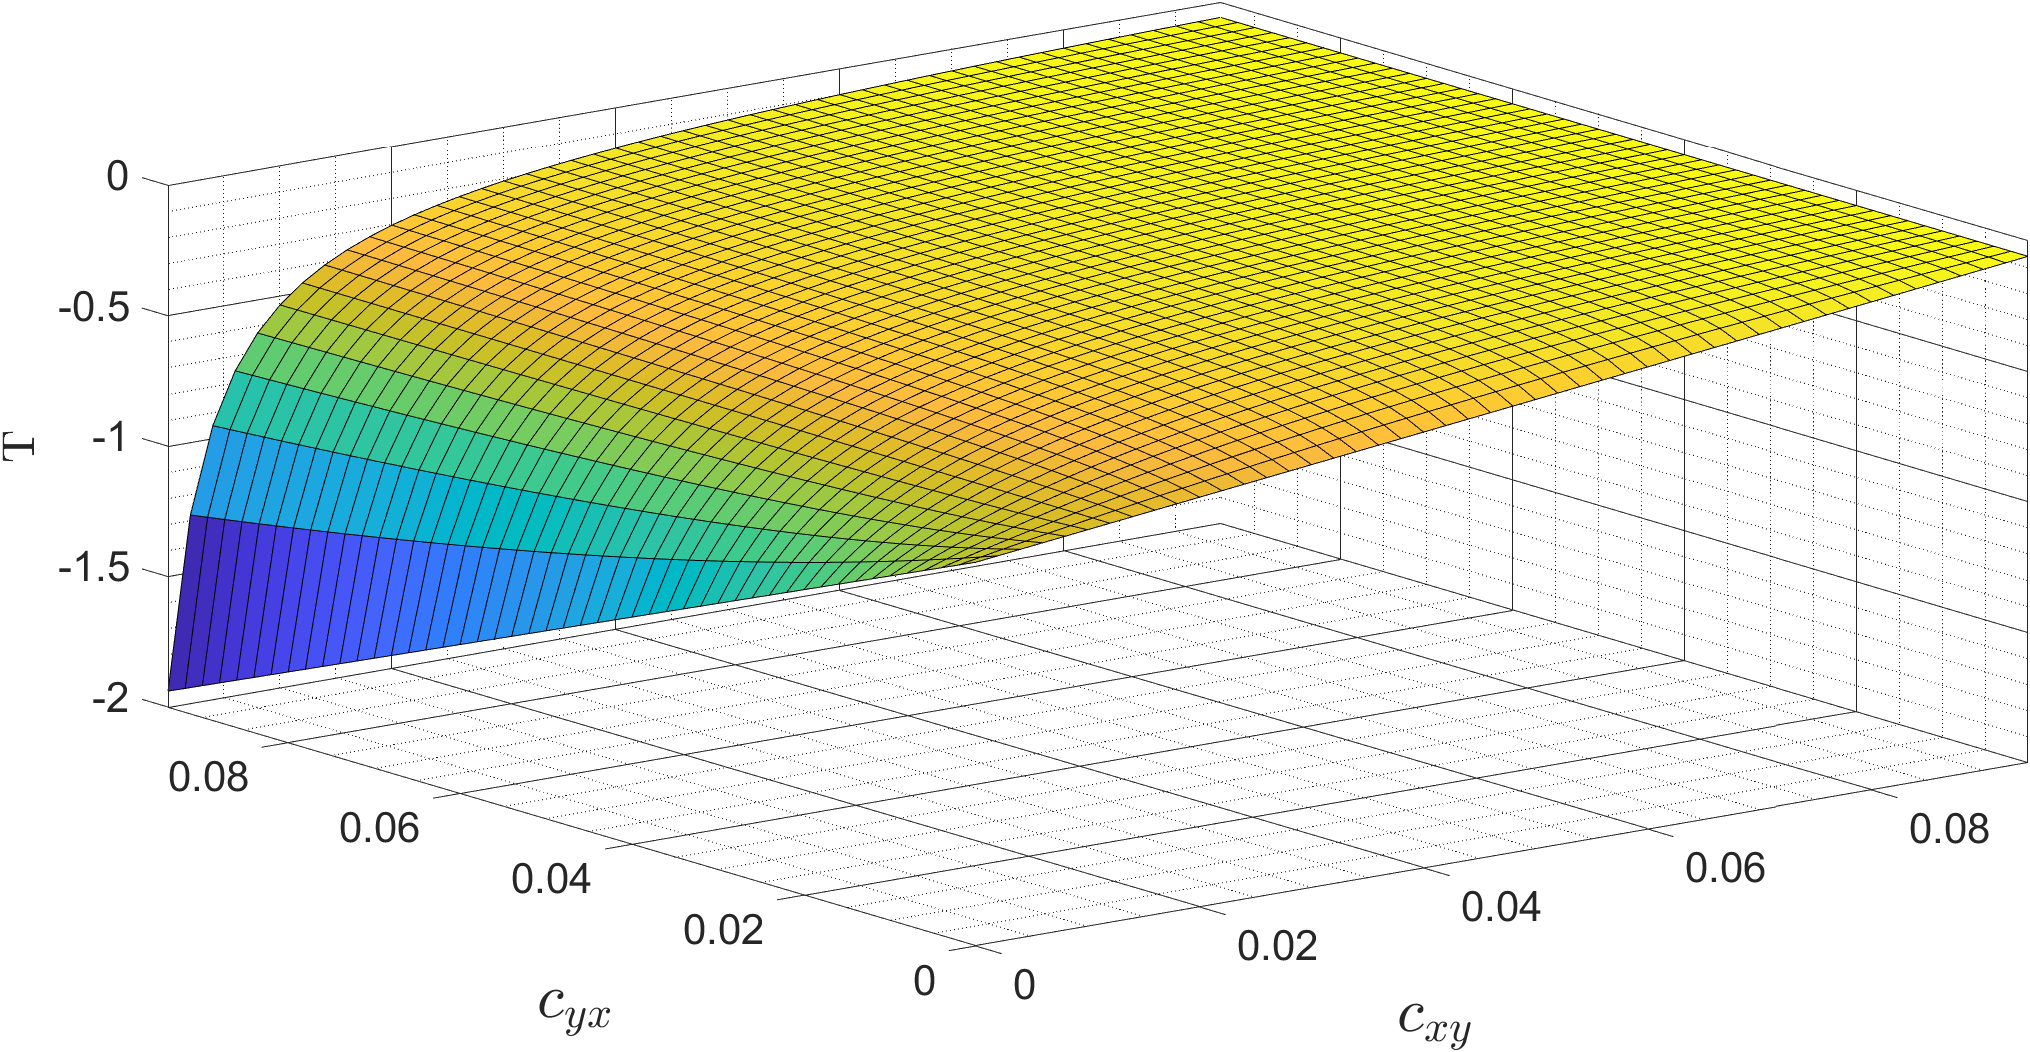
\includegraphics[width=14cm]{Pictures/Stability/Trace.png}
% \end{figure}
% \begin{figure}[H]
%     \centering
%     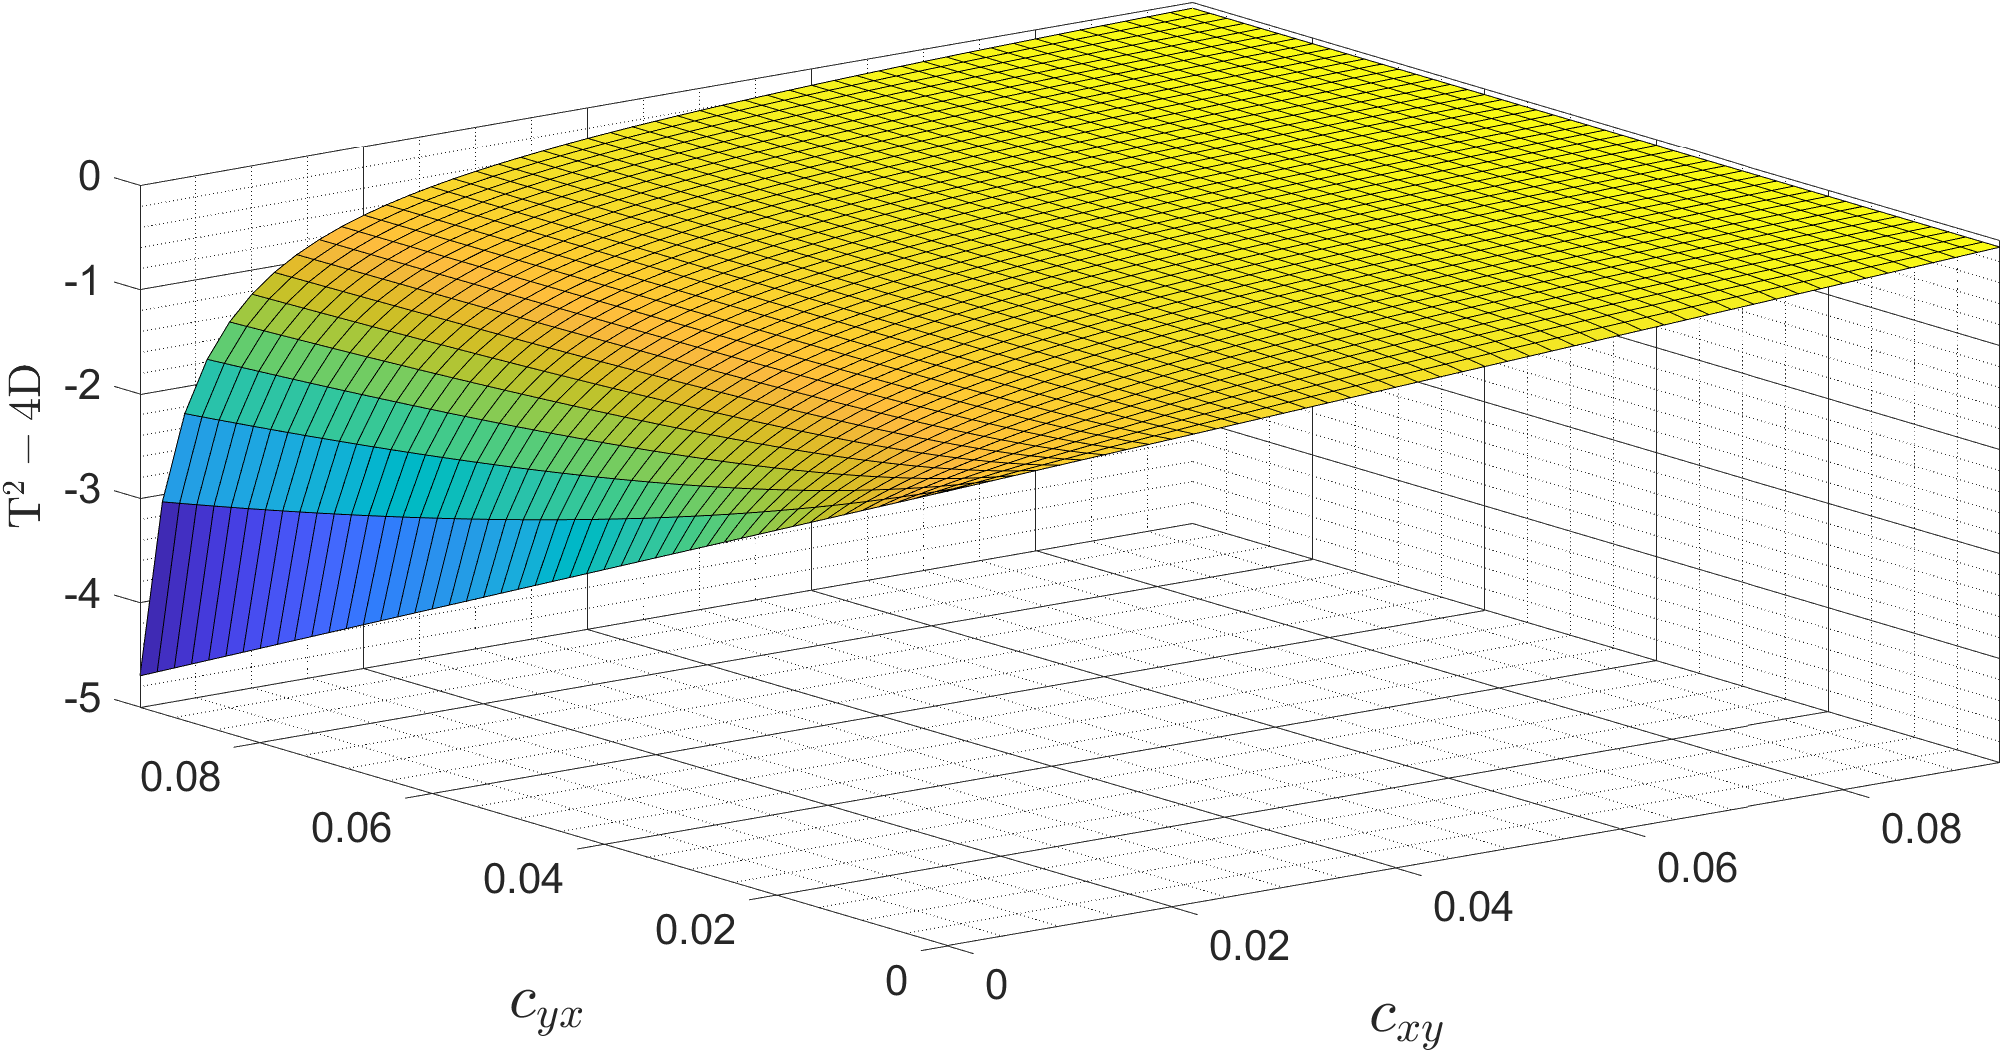
\includegraphics[width=14cm]{Pictures/Stability/Discriminant.png}
%     \caption{The graphs above are the trace and discriminant of $\displaystyle J_{(x^*_4,y^*_4)}$ for different values of the parameters $c_{xy}$ and $c_{yx}$.}
%     \label{fig:TraceDiscriminant}
% \end{figure}
% Notice that the trace and discriminant values are always negative for all $c_{xy}$ and $c_{yx}$ that belong in their constraints.
Looking at \figureautorefname~\ref{fig:TraceDiscriminant} from a top-down view, we can see which values for $c_{xy}$ and $c_{yx}$ satisfy the new constraints.

\vspace{3cm}

\begin{figure}[H]
    \centering
    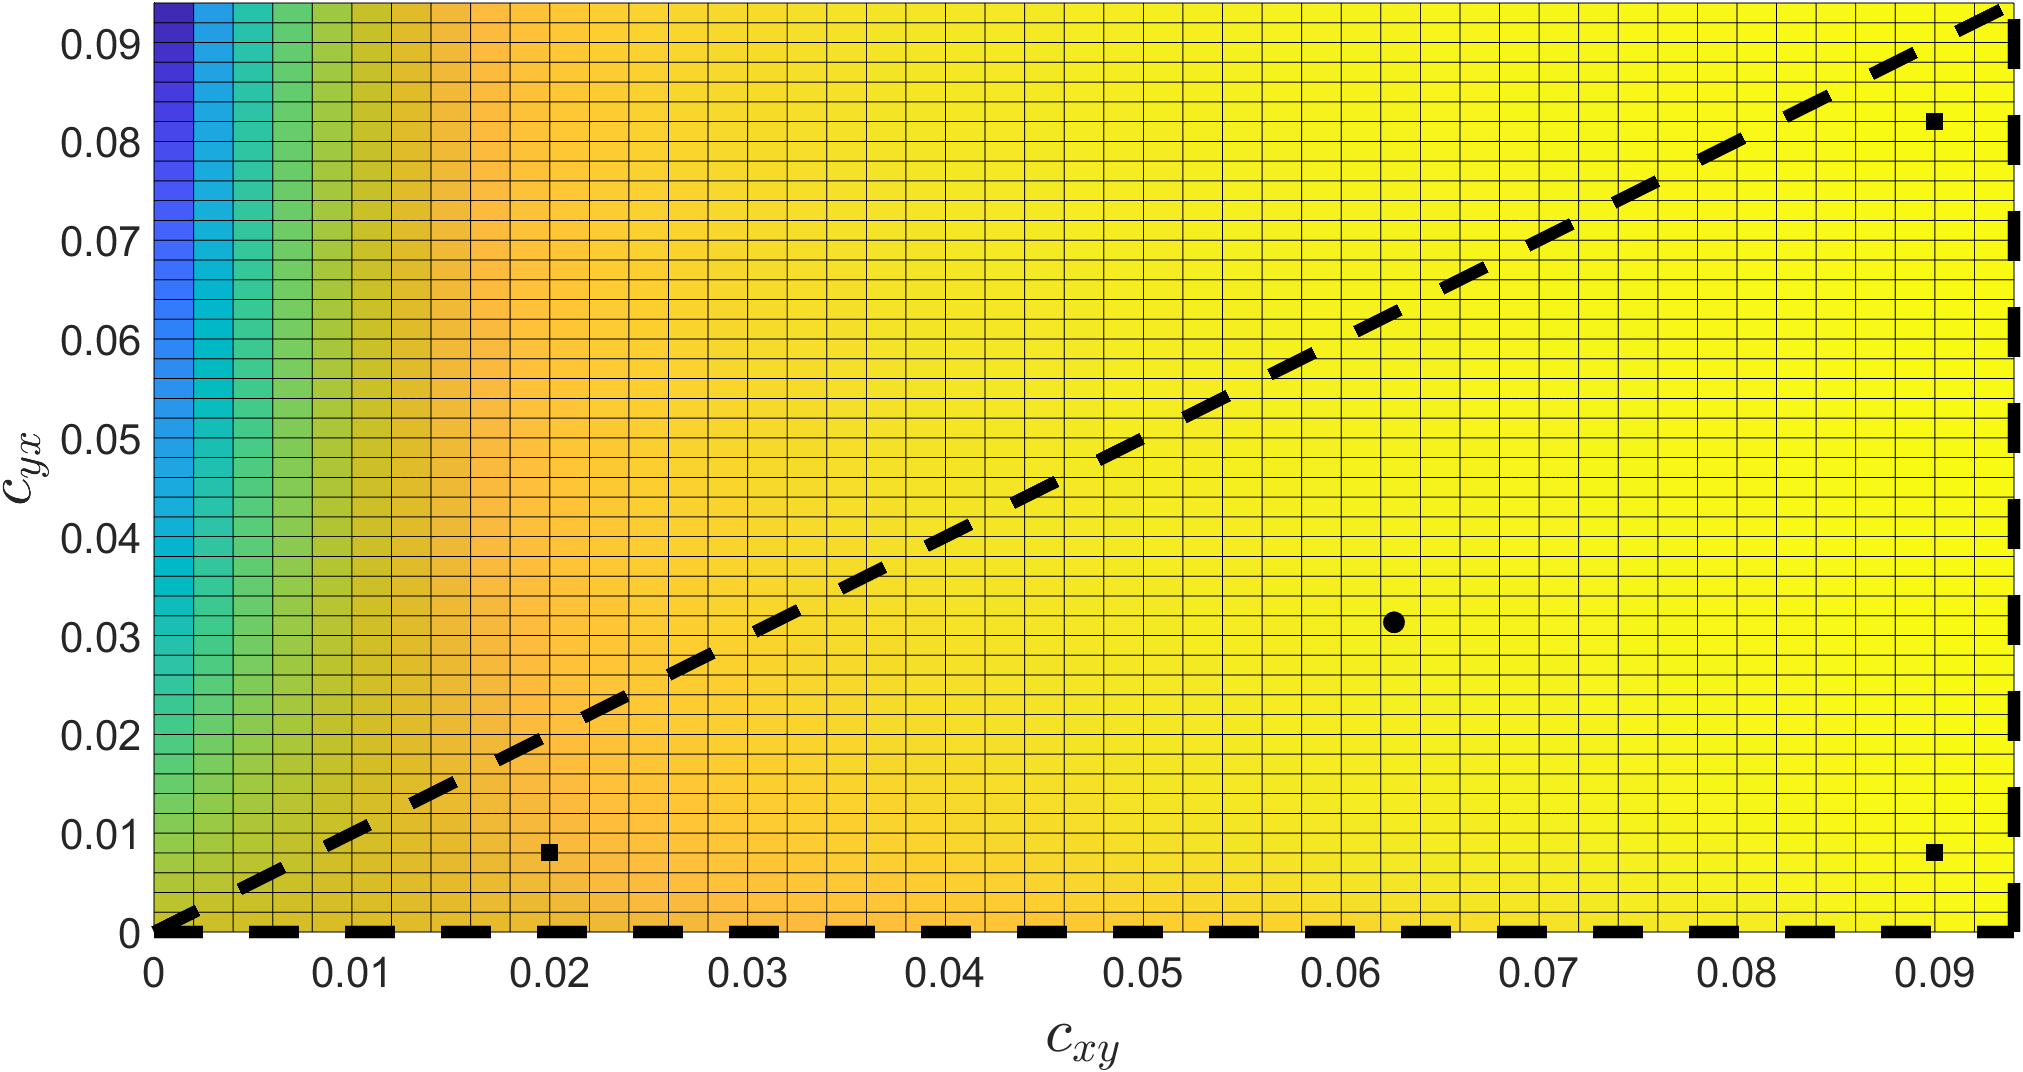
\includegraphics[width=14cm]{Pictures/Stability/TraceTopDown.png}
\end{figure}
\begin{figure}[H]
    \centering
    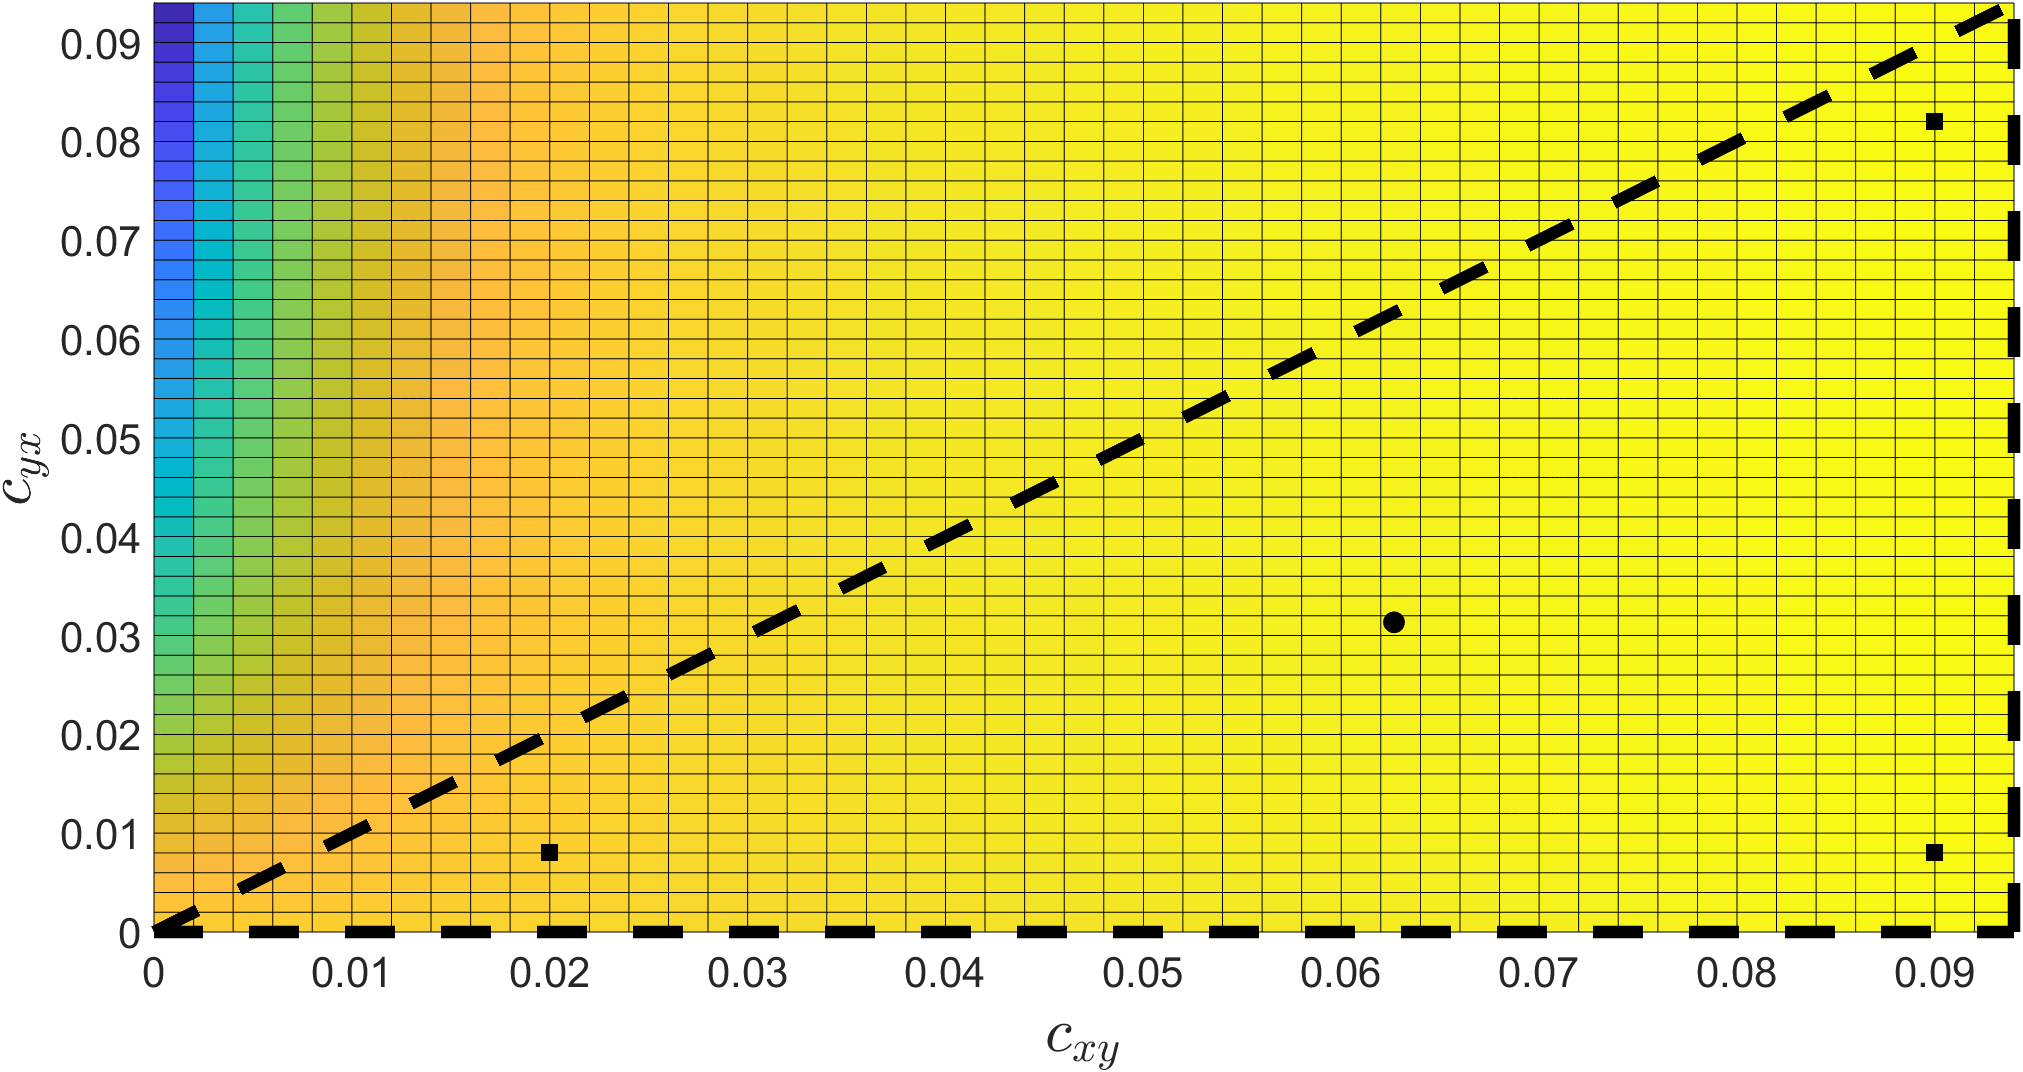
\includegraphics[width=14cm]{Pictures/Stability/DiscriminantTopDown.png}
    \caption{\singlespacing
    Top-down view of \figureautorefname~\ref{fig:TraceDiscriminant}. The points inside the right triangle are all values that satisfy the constraints of parameters $c_{xy}$ and $c_{yx}$. The right triangle's center of mass is marked with a black dot at the coordinate point $(0.0627,0.0313)$.}
    \label{fig:TraceDiscriminantTopDown}
\end{figure}
Now, we begin testing different $c_{xy}$ and $c_{yx}$ values to illustrate how different interaction rates affect the outcome of each species' population.
The values chosen for $(c_{xy},\;c_{yx})$ are $(0.02,\;0.008)$, $(0.09,\;0.008)$, $(0.09,\;0.082)$, and $(0.0627,\;0.0313)$. These pair of interaction parameters can be seen plotted in the figure above.
To compare each of the parameters, we plot the solutions to \equationautorefname~\eqref{eq:AutonomousSystemODEs}, where the brown bear population is along the y-axis, and the salmon population is along the x-axis as shown below for each pair of parameters.
\begin{figure}[H]
    \centering
    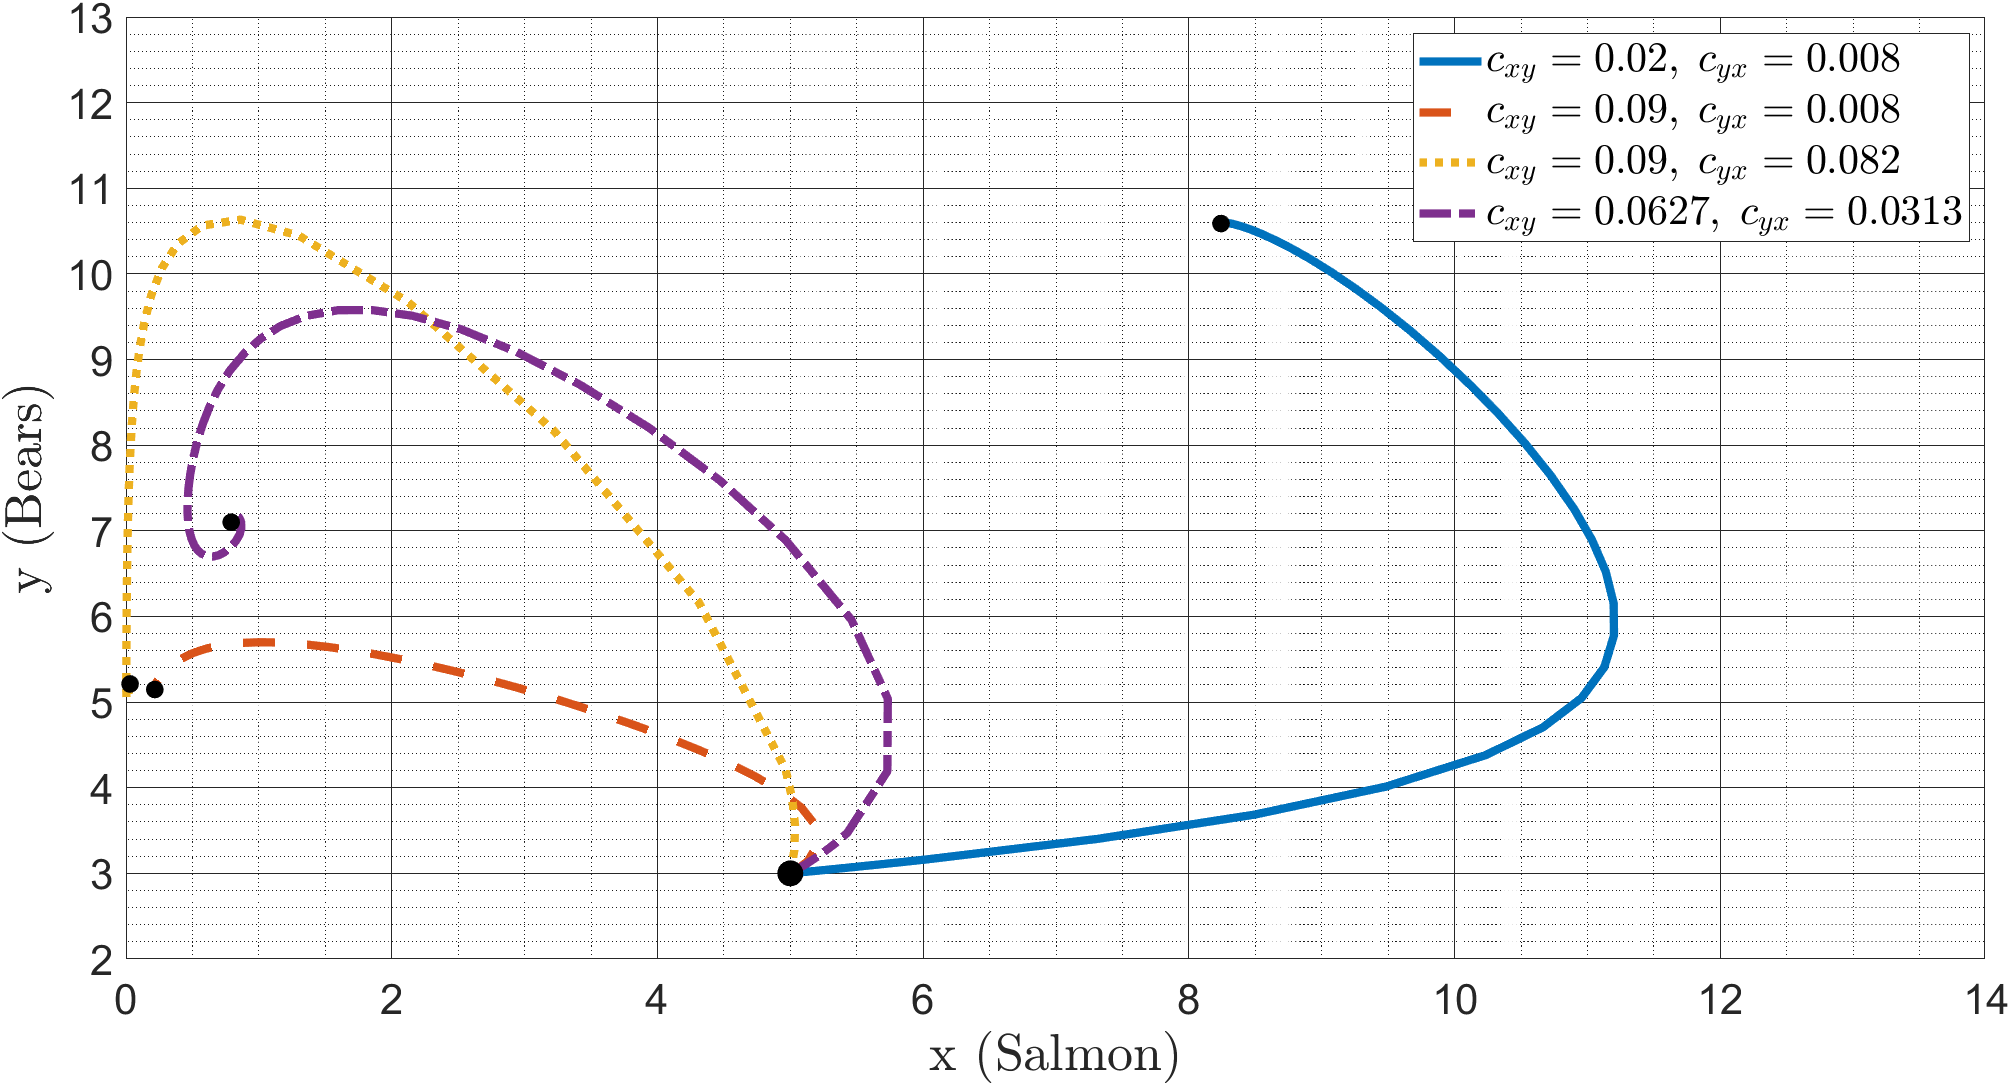
\includegraphics[width=14cm]{Pictures/Stability/SolutionsAutonomousModel.png}
    \caption{\singlespacing
    Compares the effect of different interaction rates, $(c_{xy},\;c_{yx})$, for the autonomous model, \equationautorefname~\eqref{eq:AutonomousSystemODEs}, where the initial conditions are $x_0 = 5$ and $y_0 = 3$.}
    \label{fig:SolutionsAutonomous}
\end{figure}
The graph above shows that each of these parameters affects the location of the critical point, $(x^*_4,y^*_4)$, as well as the oscillations of the populations.
We chose the initial conditions, $x_0 = 5$ and $y_0 = 3$, to illustrate the dramatic difference in interaction parameters.
When $c_{xy}$ is large, the salmon population dies off, and when $c_{yx}$ is large, the brown bear population increases faster before converging near its carrying capacity.
Lastly, when the pair of parameters is equal to the right triangle's center of mass in \figureautorefname~\ref{fig:TraceDiscriminantTopDown}, the population oscillates and converges to its critical point $(0.79,7.1)$.
We use $c_{xy}=0.0627$ and $c_{yx}=0.0313$ to represent the interaction rates of the two species for \equationautorefname~\eqref{eq:AutonomousSystemODEs} because with these parameters, the populations oscillate around their critical point much longer than the other parameters we tested, which will provide a more visible comparison for when we incorporate climate change.
So, with all the parameters selected, the solutions to the autonomous model, \equationautorefname~\eqref{eq:AutonomousSystemODEs}, with respect to time, are shown below.
\begin{figure}[H]
    \centering
    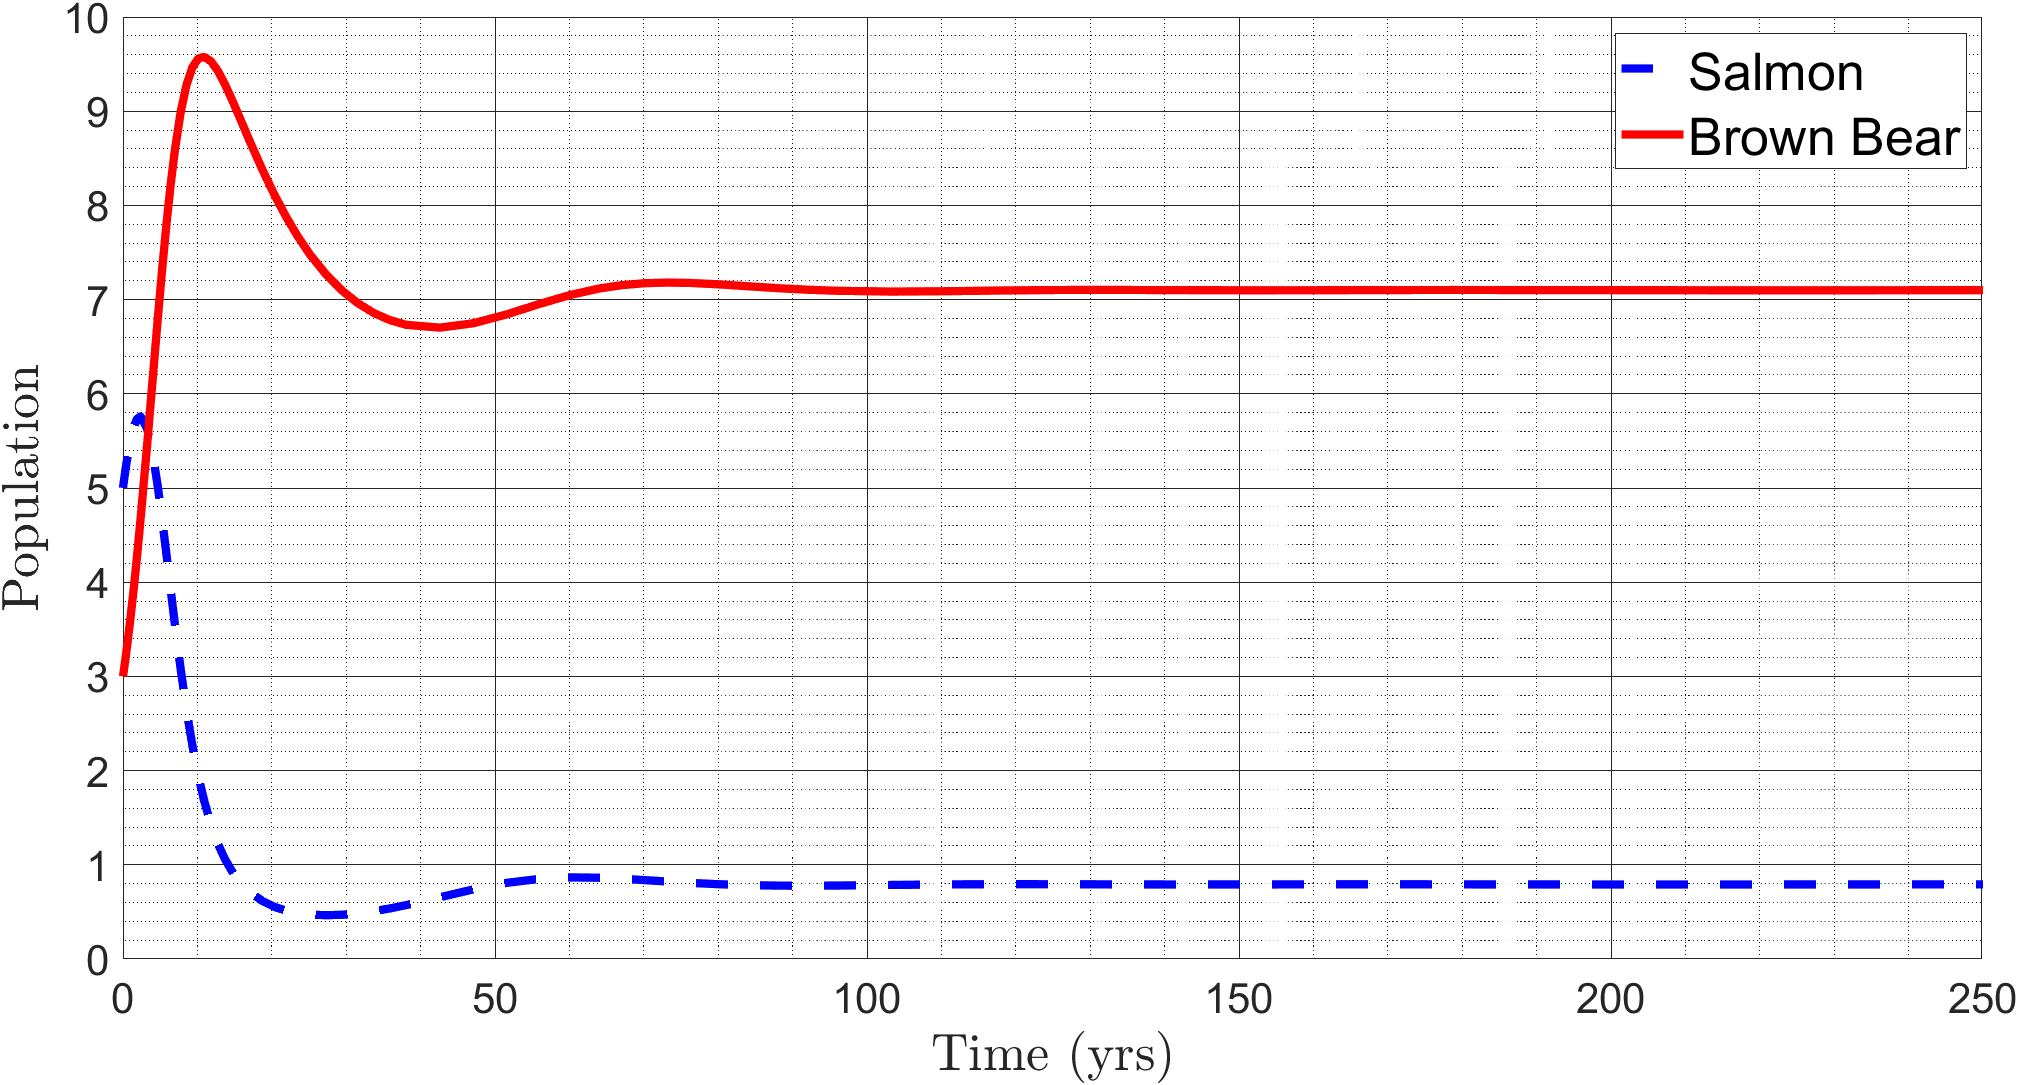
\includegraphics[width=14cm]{Pictures/System ODEs/AutonomousModelRespectTime.png}
    \caption{\singlespacing
    Plot of  the solutions to the autonomous model, \equationautorefname~\eqref{eq:AutonomousSystemODEs}, with respect to time.}
    \label{fig:SolutionsNonAutonomous}
\end{figure}
In the figure above, both populations briefly increase before changing directions and oscillating toward their equilibrium points.
Based on this figure, the brown bear population quickly overtook the salmon population, forcing the salmon near regional extinction.
